\documentclass[12pt,a4paper]{article}

% ==== Paket-Paket Ruwet Biar Berasa Hardcore ====
\usepackage[utf8]{inputenc}
\usepackage[T1]{fontenc}
\usepackage{lmodern}
\usepackage{geometry}
\usepackage{graphicx}
\usepackage{tabularx}
\usepackage{fancyhdr}
\usepackage{titlesec}
\usepackage{setspace}
\usepackage{xcolor}
\usepackage{enumitem}
\usepackage{float}
\usepackage{hyperref}
\usepackage{caption}
\usepackage{titling}
\usepackage{eso-pic}        % Tambahan untuk background
\usepackage{transparent}    % Transparansi gambar background
\usepackage{verbatim}
\usepackage{tikz}
\usetikzlibrary{positioning, arrows.meta}
\newcommand\BackgroundAllPages{%
  \AddToShipoutPicture{\BackgroundPic}
}


% ==== Geometry dan Margin ====
\renewcommand{\familydefault}{\sfdefault}
\newgeometry{top=2.5cm,bottom=3cm,left=3.5cm,right=2.5cm}

% ==== Variabel yang Bisa Diganti ====
\def\autor{Laboratorium}
\def\lab{Multimedia dan Internet of Things}
\def\departemen{Departemen Teknik Komputer}
\def\institut{Institut Teknologi Sepuluh Nopember}
\def\praktikum{Praktikum Jaringan Komputer}
\def\judul{Modul 1 – Pengenalan Jaringan}
\def\nama{I Gusti Ngurah Opaldi Partha Dwipayana – 5024221057}
\def\tanggal{2025}

% ==== Background Setup ====
\newcommand\BackgroundPic{
  \put(0,0){
    \parbox[b][\paperheight]{\paperwidth}{
      \vfill
      \centering
      \transparent{0.1}
      
\includegraphics[width=0.5\paperwidth]{Cover/img/miot.png} % Ubah path jika perlu
      \vfill
    }
  }
}

\newcommand\BackgroundNone{%
  \ClearShipoutPicture
}

% ==== Heading Style ====
\titleformat{\section}{\normalfont\Large\bfseries}{\thesection}{1em}{}
\titleformat{\subsection}{\normalfont\large\bfseries}{\thesubsection}{1em}{}


\begin{document}

\BackgroundNone  % Hilangkan background untuk halaman judul

% ==== HALAMAN JUDUL ====
\begin{titlepage}
    \centering
    \begin{tabularx}{\textwidth}{l@{\hskip 0pt}lX}
        \raisebox{-0.5\height}{
\includegraphics[width=3cm]{Cover/img/logodepart.png}} 
        & \raisebox{-0.5\height}{
\includegraphics[width=3cm]{Cover/img/miot.png}} 
        & \raggedleft
        \begin{minipage}{0.5\textwidth}
            \raggedleft
            {\bfseries \small \autor} \\[-2pt]
            {\bfseries \small \lab} \\[-2pt]
            {\bfseries \small \departemen} \\[-2pt]
            {\bfseries \small \emph{\institut}}
        \end{minipage}
    \end{tabularx}
    
    \vspace{5cm}
    {\Huge \bfseries \praktikum \par}
    
    \vspace{2cm}
    {\LARGE \bfseries \judul \par}
    
    \vspace{2cm}
    {\Large \nama \par}
    
    \vfill
    {\Large \tanggal \par}
    
    \vfill
    
\includegraphics[width=\textwidth]{Cover/img/footer.png}
\end{titlepage}

\restoregeometry
\BackgroundAllPages
% Aktifkan background setelah halaman judul

% ==== KONTEN ====
\section{Pendahuluan}
\subsection{Latar Belakang}

Dalam era digital yang terus berkembang, kebutuhan akan infrastruktur jaringan komputer yang andal dan efisien menjadi sangat penting, terutama bagi perusahaan yang mengandalkan komunikasi data sebagai tulang punggung operasionalnya. Praktikum jaringan komputer ini dilaksanakan sebagai sarana untuk memahami dan menerapkan konsep dasar hingga lanjutan dalam perancangan jaringan, khususnya dalam konteks dunia kerja nyata.

Permasalahan yang sering terjadi di dunia industri adalah kurangnya efisiensi dalam pengalokasian alamat IP, desain jaringan yang tidak scalable, serta kurangnya pemahaman dalam routing antar jaringan. Melalui praktikum ini, mahasiswa diharapkan mampu memahami bagaimana membagi jaringan berdasarkan kebutuhan tiap departemen, merancang subnet agar tidak terjadi overlap, serta mengkonfigurasi routing agar tiap jaringan dapat saling terhubung secara optimal.

Urgensi pembelajaran ini sangat tinggi, karena hampir seluruh sektor industri dan instansi pemerintahan menggunakan jaringan komputer untuk mendukung kegiatan mereka. Selain itu, pemahaman tentang IP address, subnetting, jenis routing, hingga konfigurasi router secara langsung akan memberikan bekal praktis yang relevan dengan kebutuhan dunia kerja, khususnya di bidang IT dan jaringan.

\subsection{Dasar Teori}

Jaringan komputer merupakan sekumpulan perangkat yang saling terhubung untuk berbagi data dan sumber daya. Dalam praktik jaringan, terdapat beberapa konsep teknis penting yang mendasari pelaksanaan kegiatan ini, seperti IP address, subnet mask, routing, serta protokol jaringan.

\textbf{IP Address (Internet Protocol Address)} adalah alamat numerik yang digunakan untuk mengidentifikasi perangkat dalam jaringan. Terdapat dua jenis IP address: \textit{private} (digunakan di jaringan lokal) dan \textit{public} (digunakan untuk akses dari dan ke internet). IP address dibagi menjadi beberapa kelas, yaitu Class A, B, C, D, dan E, dan umumnya yang digunakan dalam jaringan lokal adalah kelas A-C.

\textbf{Subnetting} adalah proses membagi jaringan besar menjadi jaringan-jaringan kecil (subnet) yang lebih efisien dan aman. Subnetting memanfaatkan konsep \textit{CIDR (Classless Inter-Domain Routing)} yang dituliskan dalam notasi prefix, misalnya /24, /25, dan sebagainya.

\textbf{Routing} adalah proses meneruskan paket data dari satu jaringan ke jaringan lain. Routing terbagi menjadi dua jenis utama: \textit{Static Routing} dan \textit{Dynamic Routing}. Static routing dilakukan secara manual, cocok untuk jaringan kecil dan tetap. Dynamic routing menggunakan protokol seperti RIP, OSPF, atau BGP untuk menyesuaikan rute secara otomatis, cocok untuk jaringan besar dan kompleks.

\textbf{Kabel LAN (Local Area Network)} adalah media transmisi fisik yang menghubungkan perangkat jaringan. Proses \textit{crimping} digunakan untuk membuat kabel LAN, baik dalam konfigurasi \textit{Straight-Through} (menghubungkan perangkat berbeda) maupun \textit{Crossover} (perangkat sejenis), sesuai standar T568A dan T568B.

Pemahaman terhadap teori-teori ini penting sebagai fondasi dalam membangun jaringan komputer yang efisien, aman, dan scalable, serta menjadi bekal utama dalam pelaksanaan praktikum ini.

\section{Tugas Pendahuluan}

\subsection*{1. Perencanaan Alokasi IP Address}

Dalam merancang jaringan internal perusahaan, hal pertama yang dilakukan adalah mengalokasikan IP address berdasarkan jumlah perangkat yang digunakan oleh setiap departemen. Dengan menggunakan teknik subnetting, kita dapat menentukan prefix (CIDR) yang sesuai agar jumlah host mencukupi tanpa memboroskan IP address.

\begin{table}[H]
\centering
\begin{tabular}{|l|c|c|l|l|}
\hline
\textbf{Departemen} & \textbf{Perangkat} & \textbf{Prefix} & \textbf{Rentang IP} & \textbf{Broadcast} \\
\hline
Produksi & 50 & /26 & 192.168.1.0 – 192.168.1.63 & 192.168.1.63 \\
Administrasi & 20 & /27 & 192.168.1.64 – 192.168.1.95 & 192.168.1.95 \\
Keuangan & 10 & /28 & 192.168.1.96 – 192.168.1.111 & 192.168.1.111 \\
R\&D & 100 & /25 & 192.168.1.128 – 192.168.1.255 & 192.168.1.255 \\
\hline
\end{tabular}
\caption{Alokasi IP Address Tiap Departemen}
\end{table}

Penggunaan prefix CIDR dilakukan dengan mempertimbangkan jumlah perangkat + buffer 2 IP (untuk network address dan broadcast). Dengan ini, seluruh departemen mendapatkan subnet yang sesuai kebutuhannya tanpa overlap.

\subsection*{Total Subnet dan Network Address}

Total subnet yang diperlukan adalah empat, disesuaikan dengan jumlah departemen. Semua subnet diambil dari blok IP 192.168.1.0/24, yang kemudian dibagi dengan CIDR sebagai berikut:

\begin{itemize}
\item \textbf{Subnet Produksi:} 192.168.1.0/26, untuk 62 host.
\item \textbf{Subnet Administrasi:} 192.168.1.64/27, untuk 30 host.
\item \textbf{Subnet Keuangan:} 192.168.1.96/28, untuk 14 host.
\item \textbf{Subnet R\&D:} 192.168.1.128/25, untuk 126 host.
\end{itemize}

Setiap subnet dipilih agar efisien dan tidak tumpang tindih. Penggunaan blok 192.168.1.0/24 memungkinkan pembagian subnet yang optimal dengan CIDR fleksibel.

\subsection*{2. Skema Topologi (Deskripsi Teks)}
Topologi jaringan menggunakan satu router utama yang menghubungkan semua subnet dari masing-masing departemen. Tiap departemen dihubungkan melalui interface router atau melalui switch terpisah. Deskripsinya sebagai berikut:
\subsection*{Diagram Topologi (Visualisasi)}

\begin{figure}[H]
\centering
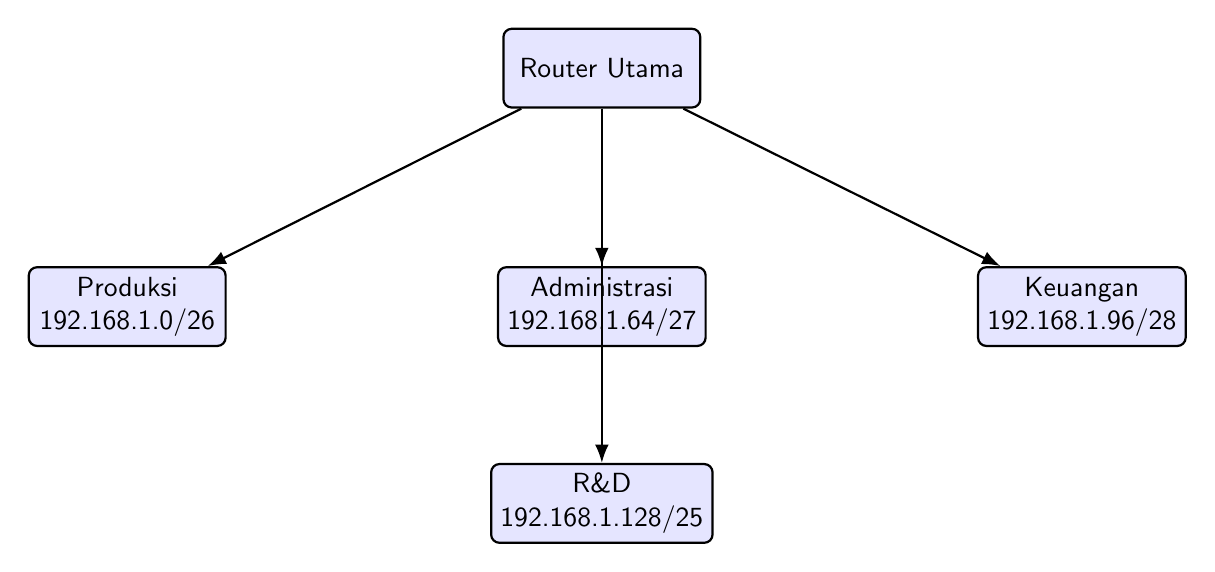
\begin{tikzpicture}[
  device/.style={rectangle, draw, thick, rounded corners=3pt, minimum width=2.5cm, minimum height=1cm, text centered, fill=blue!10, align=center},
  link/.style={-Latex, thick}
]

% Nodes
\node[device] (router) {Router Utama};
\node[device, below left=2cm and 3.5cm of router] (produksi) {Produksi\\192.168.1.0/26};
\node[device, below=2cm of router] (admin) {Administrasi\\192.168.1.64/27};
\node[device, below right=2cm and 3.5cm of router] (keuangan) {Keuangan\\192.168.1.96/28};
\node[device, below=4.5cm of router] (rnd) {R\&D\\192.168.1.128/25};

% Connections
\draw[link] (router) -- (produksi);
\draw[link] (router) -- (admin);
\draw[link] (router) -- (keuangan);
\draw[link] (router) -- (rnd);

\end{tikzpicture}
\caption{Diagram Topologi Jaringan Antar Departemen}
\end{figure}


Dengan topologi ini, komunikasi antar jaringan dilakukan melalui router, dan setiap jaringan memiliki isolasi IP-nya masing-masing.

\subsection*{3. Tabel Routing}

Routing diperlukan agar antar subnet bisa saling terhubung. Dalam kasus ini, karena semua jaringan terkoneksi pada router yang sama, kita bisa menggunakan static routing untuk mendefinisikan jalur komunikasi antar subnet.

\begin{table}[H]
\centering
\begin{tabular}{|l|c|c|l|}
\hline
\textbf{Destination} & \textbf{Prefix} & \textbf{Gateway} & \textbf{Interface} \\
\hline
192.168.1.0 & /26 & - & eth1 \\
192.168.1.64 & /27 & - & eth2 \\
192.168.1.96 & /28 & - & eth3 \\
192.168.1.128 & /25 & - & eth4 \\
\hline
\end{tabular}
\caption{Tabel Routing antar Subnet}
\end{table}

Karena tidak menggunakan router ganda atau interkoneksi lintas router, gateway tidak perlu ditentukan secara eksplisit — cukup arahkan ke interface yang sesuai. Routing ini dapat ditambahkan secara manual di sistem operasi router seperti MikroTik atau Cisco.

\subsection*{4. Jenis Routing yang Digunakan}

Routing yang digunakan dalam skenario ini adalah \textbf{Static Routing} dikombinasikan dengan \textbf{CIDR}. Static Routing dipilih karena jumlah jaringan masih sedikit dan topologinya sederhana, sehingga tidak memerlukan konfigurasi dinamis. Konfigurasi manual bisa dilakukan dengan mudah dan hasilnya lebih stabil serta aman.

CIDR digunakan karena subnetting yang dilakukan tidak mengikuti aturan classful IP address. Dengan CIDR, kita bisa menentukan prefix secara fleksibel sesuai kebutuhan host per subnet, misalnya /25, /26, /27, dan /28.

Apabila di masa depan jaringan menjadi lebih kompleks, penggunaan \textbf{Dynamic Routing} seperti OSPF atau RIP bisa dipertimbangkan untuk menyederhanakan manajemen routing dan mendukung jaringan yang scalable.


\end{document}
